\section{Introduction}

All sectors of society depend on properly functioning networks.  Further, both the complexity and requirements of these networks are increasing as more devices come online and richer services move to the cloud.  Unfortunately, network errors routinely lead to costly downtime~\cite{mahajan+:bgp-misconfiguration,feamster+:rcc,batfish,dc-failure-study}.
Figure~\ref{fig:network-downtime} reports the results of a Juniper
study on network outages.  It shows that human error, which often occurs in configuration or planned maintenance of networks, is the single largest cause of outages. 
Anecdotally, the evidence is equally compelling.  For instance, recent misconfigurations at
Time Warner led to an hour-long, nation-wide outage of their backbone network~\cite{time-warner} and at United led to temporary suspension of all US flights in July 2015~\cite{united}.

One fundamental reason for these misconfigurations is the
mismatch between the intended high-level
policies and the low-level configurations.  On the one hand, most routing policies involve
network-wide properties:  never announce a particular destination externally, isolate two subnetworks from one another, prefer traffic through a transit customer over a transit provider, etc.
On the other hand, these policies must be implemented via hundreds of low-level configuration directives at each individual router in the network.  Typically, operators do their job by manually
decomposing their network-wide policy into a set of low-level configurations,
one per device.  As a result, errors range from simple consistency issues (community values do not match) to more subtle scenarios (misconfigured ACLs causing intermittent disconnectivity)~\cite{feamster+:rcc,batfish}.

%\begin{figure}[t]
\begin{wrapfigure}{R}{0.4\textwidth}
  \centering
%  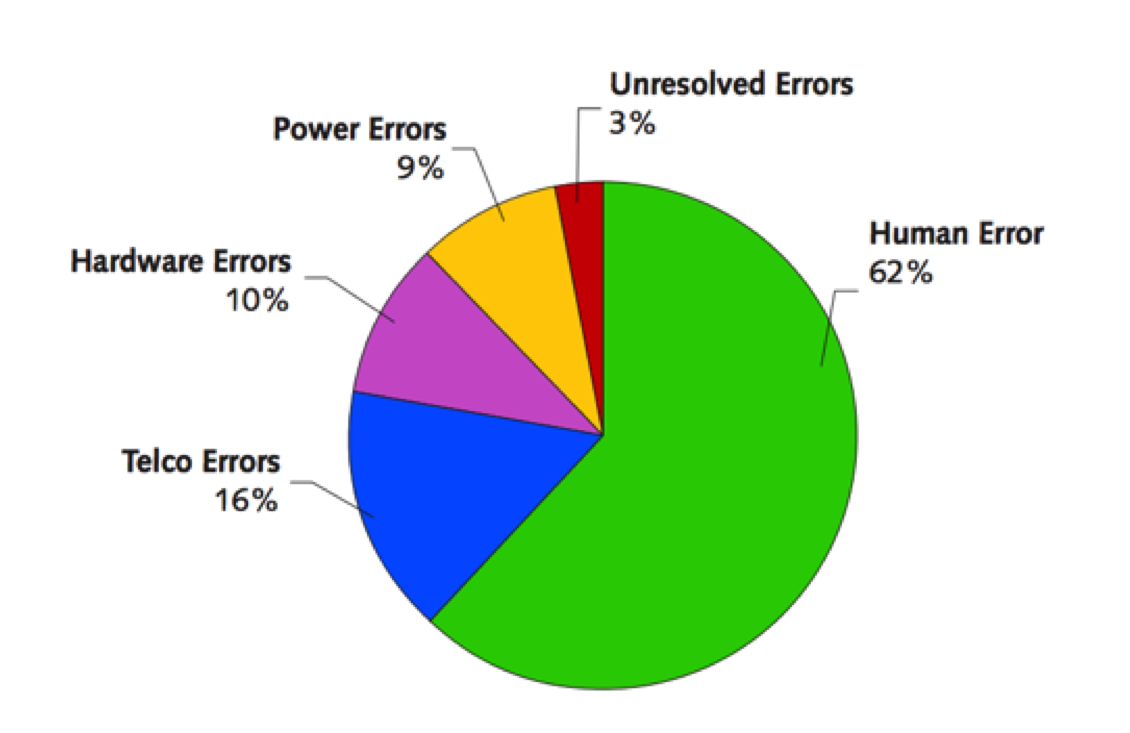
\includegraphics[width=.45\textwidth]{figures/errors1}
%  \hspace{1cm}
  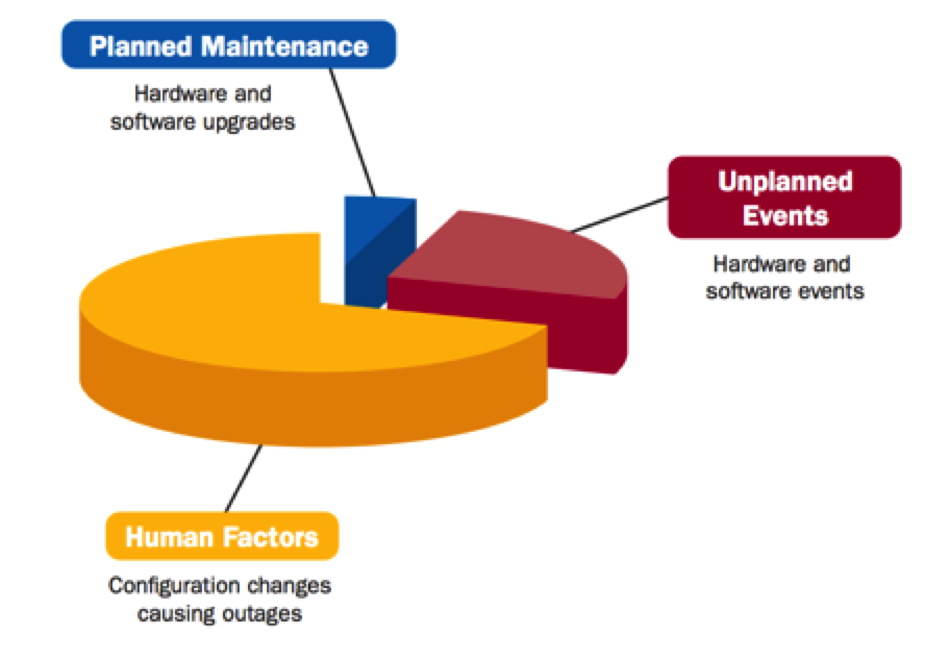
\includegraphics[width=.35\textwidth]{figures/errors2} \\
%  (a)  \hspace{3in} (b)
  \caption{
%Two studies on network downtime:  (a) From the Yankee group (2002),
%roughly 60\% of network downtime is caused by human error; (b) 
Juniper study~\cite{juniper-study}: 50-80\% of outages are the result of human error.}
  \label{fig:network-downtime}
\end{wrapfigure}
%\end{figure}

% It is well known that the fundamental problem is caused by programming individual router configs device by device to implement a network-wide policy, and % this process, like assembly language coding, is fraught with peril.  Common errors in manual BGP configuration setting range from simple consistenc
 % % (community values do not match) to complex reasoning (failure In backup only triggered after failure). 
%Networks are highly complex, distributed systems that often involve both 
%hardware and software, hundreds, thousands or more different devices, and
%many different interacting protocols and services.
%For years, we have known that managing and configuring
%such systems reliably is extremely difficult and yet crucial to our modern
%economy, government, national defense, and everyday life.  
%While there are many different causes of network downtime, ranging
%from hardware errors to power failures to bugs in embedded software,
 %A few years ago, YouTube was taken
%offline for two hours when Pakistan Telecom erroneously claimed to be
%a legitimate destination for YouTube traffic, and Hong Kong-based
%PCCW, which services Pakistan Telecom failed to drop the erroneous
%messages~\cite{pakistan-youtube}.  Before that, a Turkish telecom
%pretended to be the entire internet~\cite{pakistan-youtube}.  More generally,
%network outages serious enough to make international news continue to
%happen with great regularity~\cite{bgpmon}.

%% The solution to these problems is easy to state:
%% Simply have human operators do less of the work.  The challenge is how?  

%% \begin{quote}
%% Our central idea is to fundamentally change the level of abstraction at which
%% complex networks are configured, lifting it substantially, and having a compiler
%% fill in all of the low-level details, and finally verifying the correctness of our results.
%% \end{quote}

%% At the moment, configuring

%% Rather than have network administrators configure
%% the details of low-level protocols independently on device after device, allow administrators to
%% state the high-level properties

%One fundamental reason for these misconfigurations is the
%semantic mismatch between the intended high-level
%policies and the low-level configurations.
 %Moreover, these individual device configurations often involve more than
%one protocol, such as BGP (the Border Gateway Protocol for communicating routes between different
%autonomous systems) and OSPF (an
%intra-domain protocol for routing along shortest paths in one's own network) the protocols interact with one another.  
%In order to determine whether or not the high-level goals of a user's network-wide policy have been satisfied,
%one must reason about the interaction of protocols on individual devices and the interaction of different devices.
%In essence, the problem is akin to programming a complex, heterogenous distributed system in several
%different, low-level assembly languages, and then checking that one's high-level semantic goals have been met.

To make matters worse, networks must continue to function properly when node and link failures occur.  
%In many contexts, such as in a data center,
%there are so many devices, that failures are inevitable and frequent.  
Unfortunately, network engineers
can, at their very best, reason about their policy in the face of a very small number of failure 
scenarios.  As a result, configurations that work
correctly in failure-free environments have nonetheless been found to violate key
network-wide properties in the presence of failures~\cite{batfish}.
Finally, the described problems of network configuration affect not only the robustness of deployed networks but also the agility of an organization in making the not-infrequent larger-scale changes that are required (extending the network, upgrading equpiment, migrating to a new network architecture).

A natural solution to these problems, analogous to the trend in languages for software development over the last several decades, is to define a higher-level language for implementing desired network policies.  
% Indeed, this solution has been pursued by prior work, yet none of these languages have been widely deployed to date.  An early attempt, Routing Policy Specification Language (RPSL) was not sufficiently high level, still requiring users to manually decompose network-wide policies into router-specific configuration~\cite{rpsl}.  
Indeed, in recent years, researchers have developed a series of network-wide policy 
languages that target  software-defined networking (SDN) platforms for logically centralized control planes, such as OpenFlow~\cite{frenetic,flowlog,foster:merlin,vericon,sagiv:l,fattire,netkat,kinetic,sdn-languages}. These languages have developed intuitive, high-level abstractions for specification
of routing policy and developed algorithms that take care of many of the nitty-gritty details of
generating a low-level implementation, thereby avoiding the errors caused by
ad hoc manual configuration.
Unfortunately, these solutions do not apply to the large number of commercial clouds and 
enterprise networks that have invested in, and continue to use, distributed control planes and 
traditional routers.  These languages also cannot express critical aspects of network policy that occupy a significant portion of configuration complexity today, such as the desired network behavior in the presence of faults as well as an inter-domain routing policy (routing between one's network and its neighbors).  In other words, there are many pragmatic hurdles to surmount before
these solutions can be widely deployed in industrial settings.
%Moreover, while such languages facilitate specification of intra-domain
%routing policy (routing within one's network), they do not help users control inter-domain routing
%policy (routing between one's network and a neighbor), which occupies a significant portion of route
%configuration complexity.


Hence, the overarching goal of this project is to {\em surmount the technical challenges that impede practical deployment of high-level network abstractions}.  In preliminary work, 
the PIs have taken the first steps toward this goal by developing a
new network programming language called Propane~\cite{beckett+:propane} (winner of a SIGCOMM 2016
Best Paper Award) that borrows from SDN languages an expressive set of primitives for specifying the allowed network-wide paths.  Propane extends these capabilities to enable the specification of back-up paths via a simple form of path preferences, and allows the expression of both intra-domain 
and inter-domain routing objectives.  Crucially, rather than compiling to OpenFlow,
Propane compiles to BGP, the industry-standard, distributed, fault-tolerant and scalable inter-domain routing protocol. 
Despite these advances, it is impossible to deploy Propane in industrial settings for several fundamental reasons:

%Analogous to languages like RPSL, the Propane compiler automatically produces configurations for each router that leverage BGP to implement the desired policy.  Furthermore, the Propane compiler guarantees that the specified path preferences will be respected regardless of the link or node failures that may occur.
%And yet, Propane in its current form is not suitable for widespread deployment.  

%Propane suffers from several deficiencies that also plague the prior work and 
%must be addressed in order to make network programming languages a viable alternative 
%to the current state of the art:

\begin{description}
\item[expressiveness]  Today's low-level configuration languages provide fine-grained control over network functionality and performance.  Operators will not move to higher-level, network-wide policy languages unless they can express the subtle and complex policies that business requirements demand.  Propane's 
language is not sufficient to express several common policies used by ISPs today~\cite{routingplaybook}.

\item[intelligibility] In the near term, the low-level configurations output by the Propane compiler must be human readable and match the configuration styles in use today.  This requirement has become clear in the PIs' discussions with network engineers at two large cloud providers.  Intelligibility is necessary to give engineers confidence in the behavior of their networks, to enable configurations to be processed with a variety of existing tools, and to allow operators to directly modify configurations when necessary.  
% For instance, Network operators, especially for large, structured networks such as data centers, do not think in terms of individual devices.  Instead, they craft policy in terms of \emph{sets} of devices that
% play similar roles such as top-of-rack switch, tier-one switch, \etc and the more general \emph{topological invariants} that connect these sets (\eg, the number of edges or paths that connect elements of each set).  The output of deployable synthesis must match the cognitive models used by network operators.

\item[migration safety]  If an operator's current network is operating smoothly,
migration to a new management platform is a risk, even if that new platform
offers improved efficiency and lower future management costs.  To reduce the
risk, it is necessary to have tools that faciliate migration and verify that a new high-level policy is
functionally equivalent to the legacy configurations.

\item[incrementality] No large network is likely to switch from manual configuration to Propane in one ``flag day."   Rather, support for {\em incremental deployment} is critical, with parts of the network gradually moving to this new discipline over time.

\end{description}

%Hence, in the proposed project, we plan to design, study, build and evaluate a new platform 
%capable of (1) synthesizing multi-protocol, distributed control planes from high-level end-to-end specifications,
%and (2) helping users reliably transition from their legacy configurations to our new system.  More specifically,
%our platform will contain the following components:
%\begin{enumerate}
%\item {\bf A high-level language} with a natural and \emph{uniform} set of abstractions
%for jointly specifying \emph{intra-domain} routing constraints, \emph{inter-domain}
%routing constraints and possible \emph{back-up paths} in case of failures.
%\item {\bf Tools for automatic synthesis} of low-level, device-by-device configurations of standard
%distributed control plane algorithms from the high-level language specifications.
%\item {\bf Tools for translation of legacy configurations} into the intermediate language of our compiler.
%\item {\bf Algorithms for verification} that low-level configurations correctly implement high-level %specifications.
%The low-level configurations may have been synthesized from high-level specifications, in which case
%verification helps to double-check the correctness of our synthesis toolchain, giving network operators more
%confidence in our system.  Alternatively, the low-level configurations may have been
%translated from legacy configurations, in which case verification can help find bugs in the legacy configuration,
%or help port the legacy configuration to our new system by validating the equivalence of the legacy %configuration with 
%a new high-level specification.
%\end{enumerate}

%In order to demonstrate the feasibility of our core ideas, in preparation for this proposal, 
%we have already begun to build a prototype system called
%\Propane~\cite{beckett+:propane}. Borrowing linguistic ideas from several recent SDN languages~\cite{fattire,foster:merlin,netkat},
%\Propane users specify policy using high-level path constraints, defined using regular expressions and predicates.

%\emph{Unlike} previous SDN-oriented languages, \Propane supports the ability to specify \emph{back-up paths}, which allow users 
%to express preferences
%between routes and to indicate desired behavior in the presence of faults, and more importantly, \Propane{} does not use a 
%centralized controller.  Instead, the \Propane{}
%compiler synthesizes a collection of BGP configurations, which are used to configure conventional routers.  As such, the 
%implementation is:  (1) fully distributed, 
%(2) operates using completely standard, widely-deployed, legacy protocols, (3) can manage both intra-domain and inter-domain routing,
%(4) is highly scalable, having been used at data center and internet-scale, and (5) is fault tolerant, %offering local fault 
%detection and recovery.  However, our initial prototype supports limited user abstractions, only synthesizes configurations for a 
%single protocol (BGP), does not support verification and does not help users transition from legacy configurations to new \Propane-managed
%configurations or update their existing \Propane-managed configurations.

\paragraph*{Intellectual Merit.}
Our goal in this proposal is to develop the tools and techniques
to support high-level abstractions and {\em deployable configuration synthesis}.  Building on our preliminary work, we will develop a new platform, \Name, that addresses the deficiencies described above.  Our research has several thrusts:

\begin{enumerate}

\item {\bf Topological Abstractions:} Network operators typically craft policy in terms of \emph{sets} of devices that
play similar \emph{roles} in the network (e.g., top-of-rack switches, border routers, \etc) and the  \emph{topological invariants} among these sets (\eg, the number of edges or paths that connect elements of each set).  We will devise new abstractions that allow network engineers to easily define such roles and specify policy in terms of them.  We will then develop compilation techniques that respect these roles, producing one {\em configuration template} per role, which can be instantiated to produce the concrete configurations for each device.  
%This technique will ensure that output configurations match both the cognitive models of network engineers and their existing approach of manually implementing per-role configuration templates.  
In addition to making policies more \emph{expressive},
they will make the results of compilation more \emph{intelligible}, allowing
network operators to examine a small number of templates
rather than a vast number of individual configurations.  Templates should
also make verification more scalable.  Finally,
such infrastructure will facilitate \emph{deployment} of \Name
at large cloud providers such as Microsoft, which currently use such
template-based router configuration systems.

\item {\bf Costs, Contracts and Inter-domain Transit:} 
Existing ISPs and transit providers engage in a wide range of business
relationships with their peers, providers and customers~\cite{routingplaybook}.
In order to optimize costs in the face of such arrangements, networks
must adjust their operations according to billing cycles and traffic
volume.  To facilitate such objectives, we plan to
% build two new abstraction layers on top of our
%existing infrastructure to support such operations.  At the highest
%level of abstraction, we plan 
allow users to specify the 
\emph{financial transit contracts} that govern these relationships
directly, declaratively and precisely within a \Name policy.
These contracts will serve as input to an optimizing phase that \emph{refines}
a \Name policy by choosing routes in a \emph{time-varying} and \emph{traffic-dependent}
fashion.

%The implementation of such constraints will be engineered in terms of  
%new mechanisms for \emph{time-varying} and \emph{volume-dependent} routing 
%preferences.   

\item {\bf Back-end Diversity:} There is no ``one size fits all'' networking protocol. Propane policies compile solely to BGP, but the additional expressiveness described above, along with performance requirements and the preferences of network engineers, will demand that configurations employ multiple protocols, as is standard for manual configurations today.  We will develop algorithms that synthesize configurations employing a combination of \emph{inter-domain routing} protocols such as BGP and \emph{intra-domain routing protocols} such as OSPF and RIP.  We will also target
\emph{SDN-oriented protocols} such as OpenFlow~\cite{openflow}, P4~\cite{P4} and PIFO~\cite{pifo}, allowing networks to more easily adopt this technology when appropriate, ideally 
without operators needing to change the high-level policy specification.

\item {\bf Migration Technology:} We will develop technology to help network engineers migrate existing configurations to network-wide policies.  First, we will develop new algorithms to translate legacy configurations into a logical
representation that reflects their semantics.  Second, we will leverage modern constraint solvers to automatically compare such configurations with a proposed high-level policy, either proving equivalence or providing counterexamples that guide policy refinement.  Third, we will explore techniques to automatically infer network-wide policies from legacy configurations.

\item {\bf Mixed Verification:} Finally, we will support a mixed form of configuration, whereby some portions of the network behavior are specified with \Name and some using existing technologies.  Supporting manual configurations is essential to enable incremental deployment but also to allow an escape mechanism to specify behaviors outside the capability of \Name (just as higher-level languages allow calls to native code).  A key technical challenge is to define interfaces that specify the \emph{assumptions} and \emph{guarantees} that manual and synthesized configurations make about one another and then to verify that each side lives up to its requirements. 
%adopting and extending the notion of {\em assume-guarantee reasoning} from the literature on compositional program analysis~\cite{Jones:assume-guarantee} to support verification and synthesis for mixed configurations.  
\end{enumerate}

%% \tdm{This is a nice idea but I'm not sure where it fits.}
%% {\em Second, we will develop new algorithms that allow the \Name platform to synthesize
%% updates to low-level network configurations given a pair of old and new \Name specifications, as well as a \emph{plan} to update network devices to
%% safely transition the system from old configuration to new configuration while the system is in operation.}

\paragraph{The Team.}  Our team has the breadth of skills, backgrounds, and perspectives that will be required to accomplish the agenda set out above.  
Over the last eight years, PI David Walker and his collaborators
developed the first high-level SDN programming languages, including
Frenetic~\cite{frenetic}, Pyretic~\cite{pyretic} and NetKAT~\cite{netkat}.
He also developed the concept of consistent network updates~\cite{reitblatt+:consistent-updates},
 contributed to the design of P4~\cite{P4} and, together with PI Millstein, 
developed the award-winning
Propane system~\cite{beckett+:propane}.   Todd Millstein is an expert in automated software verification as well as techniques for static and dynamic program analysis.  He has been applying and extending these approaches to reason about various aspects of networks for the last ten years~\cite{DBLP:conf/pldi/KothariGMG07,gullible,DBLP:conf/sigcomm/KothariMMGM11,DBLP:conf/nsdi/PedrosaFKGMM15}, including development of the Batfish~\cite{batfish} and ERA~\cite{era} tools for automatic network configuration analysis and verification. PI George Varghese won the 2014 SIGCOMM lifetime award for his work on routers.  In the last five years, he has helped, with the other PIs and colleagues, create the field of network verification.  He and colleagues have created open-source verification tools for networks including Header Space Analysis~\cite{hsa} and Network Optimized Datalog (NoD)~\cite{nod}. NoD has been used by Amazon to create verification tools for customer-created virtual networks.  Together, the PIs cover the full spectrum of skills required for this proposal including programming
language semantics and design,
compilation,
network algorithmics,
program synthesis, and
network verification.

\paragraph{Broader Impacts.}  
Our economy, businesses, governmental and military infrastructure all depend upon having networks that function
reliably.  
%Unfortunately, current network configuration languages are
%terribly complex and difficult to reason about.  Consequently,
%operators all-too-often make mistakes when programming this critical
%infrastructure.  
The primary goal of this proposal is to develop
a path for deployment of high-level network programming abstractions that
improves the reliability of existing legacy networks and helps
transition those networks in a safe and reliable way to new management systems.

\noindent
{\bf Cloud Deployment:}  We will work with the operators of two major clouds, Microsoft Azure and Google, to test our language and system using the policies of real industrial networks, to identify the pragmatic barriers to adoption, and to deploy our system where possible. See attached letters of collaboration.
% All three PIs have a strong connection with Microsoft.  Walker, via PhD student Ryan Beckett, and MSR collaborators Jitu Padhye and Ratul Mahajan, translated a number of Azure policies into Propane in 2015 and validated his models with Microsoft operators. Millstein has collaborated with networking researchers at MSR for the last ten years and recently won an MSR Outstanding Collaborator Award. As part of this collaboration, Millstein's Batfish~\cite{batfish} tool identified several configuration errors in Azure data centers that were subsequently fixed.
%Varghese worked at MSR from 2012-2016 and continues to collaborate with his former colleagues.  We will also seek to deploy at Google: both Walker and Varghese have collaborated with Amin Vahdat, the head of networking at Google.  These two clouds are different because Azure is a public cloud while the Google cloud supports Google services; adding abstractions that cover both use cases will be an important step toward credibility.  Collaboration will be facilitated via student internships at Microsoft and Google, as we have done recently with Princeton and UCLA Ph.D.\ students Ryan Beckett and Ari Fogel.

\noindent
{\bf Broader Outreach:}  
%While Microsoft and Google will teach us a great deal, we need to learn policies from a broader set of networks.  
In order to maximize the effectiveness of our proposed research and make a broader
impact, we must educate both students and industry alike.  To do so,
we will engage in industry outreach, by organizing a workshop under
the umbrella of the newly-formed
Cornell-Princeton Center for Network Programming (CNP)~\cite{center-for-network-programming}.
Modelled after the inaugural CNP summit in New York, which drew roughly 50
invitation-only participants from the North-East, including industry participants
from networking, hardware, software and financial companies, our workshop will 
encourage academics to engage with industry via panel
discussions, technical talks and informal discussions.  

%As we have done in the development of our prior work on Propane~\cite{beckett+:propane} as well as tools such as Batfish~\cite{batfish}, we will obtain iterative feedback from network engineers and operators to ensure that our research results will meet their needs.  Indeed, Batfish identified serious misconfiguration errors in several real-world enterprise and cloud networks that were subsequently fixed.  Also as in our prior work, we will make our tools publicly available for use by other researchers and practitioners.

\noindent
{\bf Education:} 
%We also plan on having educational impact in various ways.  
High-level network engineers will require a mix of skills in 
formal methods and network protocols.  We will develop modules for
both graduate and undergraduate networking classes to expose students
to these ideas.
%Varghese and Millstein are co-teaching a seminar class at UCLA in Fall 2016 on ``Verification, Synthesis, and the Creative Habit" to jump-start a formal graduate class.  
%We hope to
%produce future network engineers with interdisciplinary skills in verification
%and programming languages.
%Those core
%courses are taken by both programming languages students and students
%in other disciplines to cover PhD breadth requirements.  
%By
%demonstrating how PL techniques can be used to facilitate software
%development in other domains, we hope to increase engagement of
%students from other disciplines.
In addition,
the PIs have a track record of engaging undergraduates in research, often resulting in publications.  This project will allow us to engage undergraduates in interdisciplinary
research that applies programming language techniques, such as
automated verification and optimizing compilation, to problems in the networking domain. 

\noindent
{\bf Under-represented Minorities:} Finally, the PIs have a history of engaging women and under-represented minorities in
their research projects and will continue to seek out opportunities to
do so.  

\section{Preliminary Work}
\label{sec:propane}

\begin{figure}[t]
    \centering
    \begin{minipage}{.5\textwidth}
        \centering
        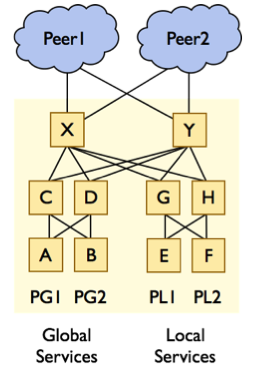
\includegraphics[width=0.6\textwidth]{figures/datacenter-topo}
        \caption{Data Center Topology}
        \label{fig:data-center-topo}
    \end{minipage}%
    \begin{minipage}{0.5\textwidth}
        \centering
\begin{mylisting}
 1. define Locality = 
 2.   {PL1 | PL2 => always(in)}
 3. 
 4. define NoTransit = 
 5.  {true =>!transit({Peer1,Peer2})}
 6.
 7. define Ownership = 
 8.  {PG1   => end(A)
 9.   PG2   => end(B)
10.   PL1   => end(E)
11.   PL2   => end(F)
12.   true => exit(Peer1 >> Peer2)}
13.
14. define Main =
15.   Ownership & Locality & NoTransit & 
16.   agg(PG, in -> out)
\end{mylisting}
        \caption{Data Center Policy}
        \label{fig:policy}
    \end{minipage}
\end{figure}

Our new ideas for deployable synthesis are best understood in the context of
our preliminary work on \Propane~\cite{beckett+:propane}. 
%Reviewers familiar with \Propane may skip to section~\ref{sec:research}, where we describe our proposed new research.  
%
\Propane allows users to program collections of routers running BGP
by writing down high-level, declarative constraints that 
describe the paths that traffic is allowed to flow along, as well
as the back-up paths to use in case of failure.  These constraints are
concise as well as {\em compositional}, allowing users to
construct complex policies
from relatively simple parts.  In fact, in studies of policy we obtained
for a data center 
and a backbone network from a large cloud provider, we have found that 
realistic
routing policy (not including definitions of prefix groups and ownership of
prefixes) that faithfully expresses the concerns of network operators
can be expressed in as little as 30-50 lines of Propane
code.  In contrast, representing the same policy in low-level BGP 
configurations requires \emph{thousands of lines of code per device}.
Some of this surprising economy of notation comes from the high-level 
abstractions we use
(regular expressions and logical predicates, which may expand exponentially
when converted into lower level abstractions such as deterministic
automata and prioritized tables); some comes from sharing
policy effectively across groups of destinations; some comes from
sharing policy across multiple devices; and some comes from the fact
that our system automatically synthesizes so many low-level details (local preferences,
community values, MEDs, import and export filters per device).  All told, 
the savings make Propane policies vastly
easier to understand, analyze, maintain and modify than traditional
configurations.

\paragraph*{Language.}
As an example, consider the idealized data center topology presented in
Figure~\ref{fig:data-center-topo}.  Here, PG1 and PG2 represent sets
of destination prefixes that supply services to the outside world (G stands
for Global and P for Prefix).  These destinations originate at top-of-rack (TOR)
switches A and B respectively.  PL1 and PL2 are local services originating
at E and F.  The data center owns and controls each of the named switches
A, B, C, \etc, and is connected to the rest of the internet via
two peers, named Peer1 and Peer2, which it does not control, but with
whom it communicates via BGP.

Figure~\ref{fig:policy} shows a \Propane specification for this data center which meets a number of objectives.  Lines 1 and 2 define a policy named \texttt{Locality}, which expresses the requirement that
the local services should be isolated from the rest of the internet.  
\Propane policies contain clauses of the form
\texttt{$X$=>$P$} where $X$ defines a set of destination prefixes and 
$P$ defines a set of ranked (acyclic) paths along which traffic may flow 
to reach the given destination.  The keyword \texttt{in} refers to
any network location that we control; the constraint \texttt{always($L$)}
defines paths that only use locations in the set $L$.  Hence, line 2
of the policy ensures traffic flowing to and from PL1 and PL2 remains within
our data center.  The \texttt{NoTransit} policy on lines 4 and 5 prohibits traffic from Peer1 to Peer2 (and vice versa) from flowing through our data center.  This policy uses the constraint 
\texttt{transit($S$)}, which defines the set of paths between members of the set $S$.
The constraint\texttt{!transit($S$)} therefore represents the complement of such a set.
The \texttt{Ownership} policy demands that any path
to a given prefix group ends at the appropriate TOR switch.  On line 12 this policy also uses a preference constraint \texttt{>>} to indicate that paths \texttt{exit}ing Peer1 from the data center are preferred to paths \texttt{exit}ing Peer2.  The \Propane compiler, described below, will ensure that this preference is respected, with traffic exiting from Peer2 only when a path through Peer1 is unavailable (e.g., due to failures).  Finally,
\texttt{Main} is defined as the conjunction of all of the previous constraints,
and in addition specifies a \emph{control constraint}.  The control
constraint \texttt{agg(PG,in->out)} demands that any announcement
for a more precise prefix, such as PG1 or PG2, be transmitted as the
more general prefix PG along any topology edge between nodes \texttt{in}
our network and nodes \texttt{out}side of our network.

%
%\begin{figure}[!h]
\begin{wrapfigure}{R}{0.5\textwidth}
%\begin{minipage}{.5\textwidth}
  \centering
  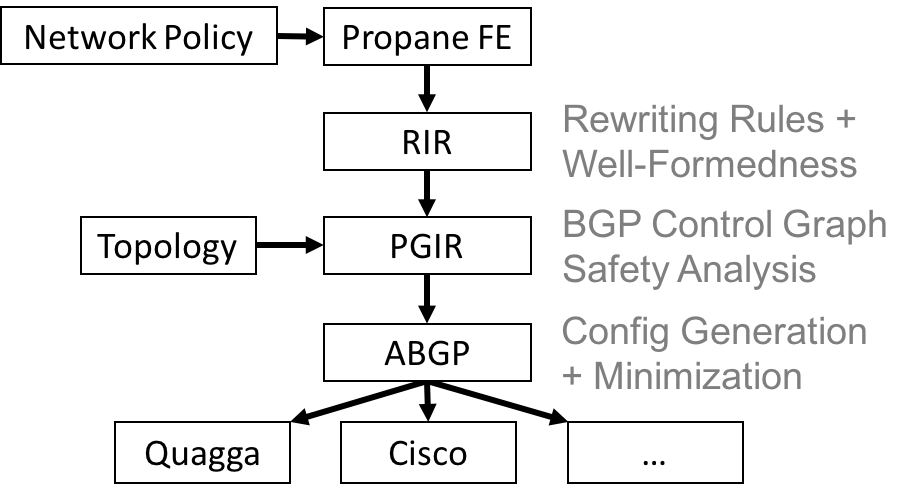
\includegraphics[width=.45\textwidth]{figures/pipeline}
%\end{minipage}
%
%% \begin{minipage}{.5\textwidth}
%% \begin{code}
%% \end{code}
%%   (b)
%% \end{minipage}
\caption{\Propane architecture.
%FE = Front End;
%RIR = Regular expression Intermediate Representation;
%PGIR = Product Graph Intermediate Representation;
%ABGP = Abstract BGP; Quagga/Cisco: Vendor-specific Router Config.
%Languages.
}
  \label{fig:pipeline}
  \vspace{-1em}
\end{wrapfigure}
%\end{figure}
%
\paragraph*{Architecture.}
Figure~\ref{fig:pipeline} presents the architecture of the
current \Propane compiler, which synthesizes low-level, device-by-device configurations
from high-level, end-to-end specifications.  
To do so, the compiler transforms the front-end (FE) specifications through
a series of intermediate languages.  The first intermediate language, the
RIR, unfolds definitions such as \texttt{end}, \texttt{transit} and \texttt{always} into raw regular expressions and merges all the constraints for a single
prefix.  

The next step is to combine information about
the user-declared policy with the network topology.
This is achieved by converting regular expressions into deterministic
automata, using standard techniques and then ``intersecting'' the graph
defined by the automaton with the graph defined by the topology.
We call this lower-level graph-based representation the \emph{product graph} (or PGIR).
Intuitively, every node in the PGIR contains both a topology location
(A, B, C, \etc) and an automaton state (q1, q2, q3, \etc).  There is an
edge from node (A,q1) to node (B,q2) in the product graph if there is
a link in the topology from A to B, and the \Propane policy states that
it is legal to progress from automaton state q1 to q2 when traversing
location B.  Hence,
the key property of the PGIR is that any path from start to final state
obeys \emph{both} the constraints of the topology and the constraints
of the policy.  As a consequence, the compiler may perform any
analyses that depends on both topology and policy using this representation.  
%For example,  
%it may determine whether node A can be reached from node B; it can determine
%what the effect of failing a particular link or topology node has on 
%connectivity; and it can determine whether BGP can implement the policy
%faithfully (not all product graph policies can be implemented faithfully).

Once various analyses have been performed on the product graph, it is
transformed into abstract BGP (ABGP), a vendor-agnostic variant of BGP.
From there, configurations for individual devices may be generated in
vendor-specific formats such as Cisco or Quagga formats.

\paragraph*{Related Work.}
The \Propane system and language design is inspired by past work on many 
recent SDN programming
languages~\cite{frenetic,pyretic,flowlog,foster:merlin,netkat,kinetic,pga}.
However, several significant differences stand out:  (1) the ability to express
both intra-domain routing and \emph{inter}-domain routing is missing in
previous SDN languages;
(2) the ability to express routing \emph{preferences} and 
\emph{back-up paths} is missing in
previous SDN languages;
and (3) the ability to compile to fully distributed control plane
protocols such as BGP, which need no centralized controller,
scale to the largest networks, and fail and recover locally.

Another related system is SDX, the software-defined exchange 
point~\cite{sdx,isdx}. This project involves design of a route server, which 
composes the routing policy from
many neighboring networks that exchange traffic
with one another.
In contrast, the goal of \Propane is to support high-level 
specification of routing policy for \emph{one}
network.  The technical challenges are different too:
\Propane compiles to traditional distributed protocols (BGP) as opposed
to infrastructure managed by a centralized route server.

RPSL~\cite{rpsl}, Nettle~\cite{nettle}, ConfigAssure~\cite{narain:lisa05,narain+:configassure}, and DADC~\cite{DADC} are languages designed to specify routing policy for distributed control planes
running legacy protocols.  RPSL uses attribute-value pairs to specify policy,
Nettle embeds router specifications in Haskell, and
ConfigAssure and DADC use logic programming
and SAT to infer parameters for configurations automatically and to ensure they
are consistent.  \Propane differs from this past work in a number of ways, but most
importantly in the kinds of abstractions provided.  In particular, \Propane supplies
a high-level constraint language that allows programmers to specify
network-wide paths and relations between paths, while this prior work 
still requires engineers to express policy and configuration on a device-by-device basis.

%% The centralized control planes of SDN, however, are not a panacea.
%% First, while many SDN programming systems~\cite{sdn-languages} provide effective \emph{intra}-domain routing
%% abstractions, allowing users to specify paths within their network,
%% they fail to provide a coherent means to specify \emph{inter}-domain routes.
%% Second, centralized control planes
%% require careful design and engineering to be robust to failures---one must ensure that all devices can communicate with the controller at all times, even under arbitrary failure combinations. Even ignoring failures, it is necessary for the control system to
%% scale to meet the demands of large or geographically-distributed networks,
%% and to react quickly
%% to environmental changes. For this challenge, researchers are exploring
%% multi-controller systems with interacting controllers, thus bringing back distributed
%% control planes~\cite{mccauley2013extending,onos} and their current programming difficulties.
%% In addition, academic
%% language design and implementation efforts have not kept pace.  For instance, work on many
%% experimental SDN languages~\cite{frenetic,flowlog,vericon,merlin,netkat,kinetic,pga} has not yet shown how to implement fault tolerant
%% multi-controller systems that support their high-level abstractions efficiently.



\section{Research Agenda}
\label{sec:research}

Our proposed \Name system will exploit infrastructure we have developed for \Propane
but will tackle a range of key new technical challenges that impede practical deployment today.

\subsection{Topological Abstractions}

\begin{wrapfigure}{R}{0.15\textwidth}
  \centering
  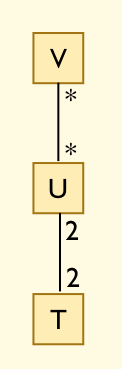
\includegraphics[width=.1\textwidth]{figures/abstract-topo}
\caption{Abstract topology with multiplicities.}
  \label{fig:abstract-topo}
  \vspace{-1em}
\end{wrapfigure}

%\paragraph*{New Topological Abstractions.}
In the previous section, we gave an example of a \Propane policy for
controlling data center routing.  In that example, the network operator
referred to individual switches by name (A, B, C, \etc).  However,
this idealized example involved a network with only 10 switches.  In
contrast, real data centers may have hundreds of switches.  In order to
manage networks at this scale, it is not effective to define policy in
terms of individual devices.  Operators must think 
in terms of \emph{groups} of devices that have similar roles:  top-of-rack switch,
tier-one switch, \etc.  Moreover, in order to plan policy and reason about
fault tolerance, operators rely on \emph{invariants} pertaining to the 
connectivity properties of these groups.  
In order to support practical policies for large networks, \Name will extend
\Propane's specifications to support
new topological abstractions of this kind.

One interesting source of inspiration for topology abstractions is,
perhaps surprisingly, the
\emph{memory analysis literature} from the programming languages 
community (\eg, Sagiv \etal~\cite{sagiv+:shape-analysis}).
Memory analysis (and alias analysis) involves analyzing programs
and inferring the shapes (often variations on lists, trees and graphs)
of data structures.  In order to make memory analysis tractable, 
the potentially infinite number of memory shapes must be collapsed into
some tractable representation.  Similar representations may be used for
describing network structures, which like program memory are structured
graphs. In particular, we believe memory
abstractions involving \emph{multiplicities} may form an effective and
novel foundation for describing classes of networks. 

As an example, consider again the data center topology presented in
Figure~\ref{fig:data-center-topo}.  This topology has three tiers of
switches, and connectivity between the layers follows fixed rules,
as is commonly the case.  In order to represent such a network,
we can represent all nodes in each tier using a single, abstract group
node and represent the edges between nodes using multiplicities.
Figure~\ref{fig:abstract-topo} presents one way of doing this.
Here abstract topology node T represents the set of concrete nodes
A, B, E and F --- T plays the ``role'' of top-of-rack switch.  Likewise,
U represents concrete nodes C, D, G and H and V represents X and Y.
Here the multiplicity \texttt{2} annotated on the edge from T to U but closer
to T indicates there are two edges extending from \emph{each} node
represented by T.  Likewise, the 2 annotating the edge coming
in to U from T represents the fact that each U node has 2 connections
to each T node.  The \texttt{*} muliplicities indicate that all nodes
represented by U are connected to all nodes represented by V and vice
versa.  The reader can verify that the concrete topology satisfies the
stated invariants --- a first research task is to develop efficient algorithms
that can check such invariants automatically in the general case.

\begin{wrapfigure}{R}{0.4\textwidth}
  \centering
  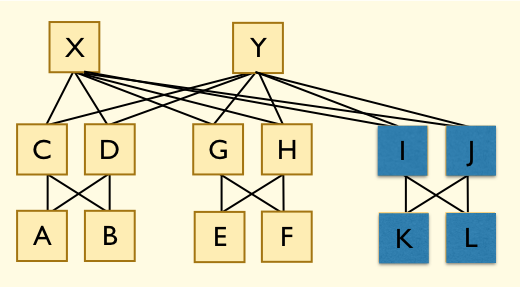
\includegraphics[width=.35\textwidth]{figures/extended-topo}
\caption{Extended data center topology.}
  \label{fig:extended-topo}
  \vspace{-1em}
\end{wrapfigure}
There are a variety of ways to use such abstractions in the process of
programming, synthesis, maintanence and verification.  As mentioned above,
such abstractions more closely match current operator practice when
reasoning about and planning data center policy.  In addition, such
abstractions can capture \emph{classes} of concrete network topologies.
For instance, if we wanted to extend our data center with an additional pod,
as shown in Figure~\ref{fig:extended-topo}, we could do so and 
the extended topology also
matches the given abstract topology.  Consequently, a policy written in
terms of our abstract topology could be applied to \emph{either} concrete
data center topology.  This fact means that it is possible to work hard
to get routing policy right \emph{once} but then potentially \emph{reuse} that
work effectively over many data centers with related shapes, or when more
equipment is provisioned in an existing data center.  In essence,
such abstractions provide a new kind of modularity for network programs.

Of course, to capture rich classes of networks with a variety of
striping patterns, inter-connections, and connectivity
invariants
we will likely need many more different kinds abstractions than are
shown in Figure~\ref{fig:abstract-topo}.  In particular, when we examine a wide range of network
topologies~\cite{al-fares:data-center-architecture,f10,quasi-fat-trees,aspen-trees,jellyfish,dcell}, 
we believe we may need multiplicities on nodes (constraining the
number of nodes in an abstract node or pod), relations between 
multiplicities (e.g., $n \geq 2$
to ensure that nodes are connected by at least two edges to other parts of the data center), probabilistic relations (to describe randomized network
designs like Jellyfish~\cite{jellyfish}) and nested abstractions (to describe the
hierarchical structure of designs such as DCell~\cite{dcell}).  

%\paragraph*{Compilation and analysis with abstract topologies.}
Our new abstractions will also be an important component of the implementation
infrastructure of \Name. 
Many large cloud providers, such as Microsoft, define policy based on
\emph{templates}, with one template for each role or abstract group of
routers.  The parameters of each template may be instantiated to generate
concrete router configurations for each router in the group.
Indeed, there are a variety of tools available, such as Hatch~\cite{hatch}
and Thwack~\cite{thwack},
to help with the definition and sharing of such templates.
In order for \Name to be deployed in the context of existing template-based infrastructure,
it will be necessary to revisit \Propane's compilation algorithms so
that policy expressed over abstract topologies generates appropriate
templates rather than concrete configurations.  Generating templates will
also help network operators validate the output of the \Name compiler:
they will only have to examine a small number of template files, one for
each role, rather than one for each device.

Finally, we will explore techniques for reasoning about abstract topologies in order to verify various kinds of properties.
For instance, operators may like to know whether two destinations
are reachable from one another, or for security purposes, whether
two destinations are isolated from another, or how many failures
it takes to partition a network or make certain destinations unreachable.
One the positive side, abstract topologies are much smaller than concrete
topologies --- this may be a major advantage, allowing sophisticated 
analyses to execute much more quickly on large networks.  However, the
abstractions also make the analysis algorithms more challenging, as they must now prove properties over entire \emph{classes} of networks instead of
individual \emph{concrete} networks.  We believe we will be able to exploit
ideas from the field of \emph{abstract interpretation}~\cite{cousot+:ai} (the subfield of
programming language research that deals with the science 
of analyzing abstract structures) in defining our algorithms and in proving
them correct.  It will take significant practical and theoretical
research to develop, implement, test and prove correct the necessary 
algorithms for fault tolerance, reachability and security analysis.


\paragraph*{Related research.}
In terms of related research, the closest overlap is with the 
Condor project~\cite{condor}.  However, Condor focused on description
of topologies and then generation and testing of a finite number of
sample topologies with a goal of discovering new topologies that might be 
deployed in next-generation data centers.
In contrast, our work will integrate abstract topologies into the
network programming process. Unlike Condor,
we will develop
compiler algorithms that generate router configuration templates from
abstract topoplogies and operator-level policy.  We will also 
study algorithms for verifying \emph{universal}
fault tolerance and reachability properties---\ie, properties that
hold \emph{for all} concrete
networks that inhabit a given class of topological abstractions.  Such
universal properties provide strong guarantees for classes of
related networks and future-proof networks
that may be expanded.  
Pyretic~\cite{pyretic} and NetKAT~\cite{fast-compiler} also contain sublanguages
that enable virtual networking, but their abstractions do not describe
connectivity invariants and their compilers do not perform analyses over
abstract networks or generate template-based router configurations.

Recent work by co-PI Varghese on network ``symmetry and surgery''~\cite{bjorner+:scaling-network-verification} verifies reachability properties of the data planes of very large
data centers by leveraging symmetries in the networks to  
transform them into
related, smaller networks.  The ideas
developed there may be a useful starting point for verifying properties of \Name policies on abstract topologies; we will need to extend these ideas to handle the expressive abstractions that \Name will support, such as multiplicities.  


\paragraph*{Summary of key research questions:}

\begin{itemize}
\item What abstractions help us specify invariants of common data center and ISP network topologies? How do we integrate such abstractions into the \Name system?
\item How do we compile with abstract topologies and make use of operator-friendly templates?  
\item How do we analyze properties of network policies, such as
reachability and fault tolerance, over abstract
topologies?  How do these algorithms perform?
\item What is the formal 
semantics of abstract topologies?  How do we prove our
compilation algorithms and analyses are correct?
\end{itemize}

\subsection{Costs, Contracts and Inter-domain Transit}
%% A key goal of \Name is to synthesize common policies used by Data Centers and ISPs, many of which are 
%% detailed in \cite{routingplaybook}.   In particular, we aim to add to \Name the ability to craft policy based on
%% 5 traffic (in order to reduce billing costs) which is impossible to do in \Propane.
%% \paragraph*{Traffic Engineering and Inter-domain Routing.}

Many networks have complex business relationships with their peers, providers and 
customers \cite{routingplaybook}.  Such networks must satisfy agreements to carry traffic 
while minimizing
cost, thereby maximizing their own profits. The current \Propane language does
not incorporate any information about transit costs 
and hence \Propane's compiler has no way to optimize routes to achieve these
business objectives.
Inspired in part by past domain-specific languages for specifying contracts for financial derivatives~\cite{spj+:contracts},
we will develop a sub-language that allow users to specify the
\emph{costs} associated with using different interdomain routes, the \emph{peering agreements} they
engage in, and the \emph{contracts} signed with customers or providers.  For example,
our sub-language will allow description of the common 95/5 contract~\cite{routingplaybook}.  
In this contract, customer traffic is measured at 5-minute intervals and is billed at 
some agreed upon rate X multiplied by the
volume measured during the 95th percentile interval each month.  Such contracts allow customers to burst for small
percentages of the time without suffering outsized bills.  Other common kinds of contracts include
\emph{tiered contracts}~\cite{tiered-isp-contracts}, in which customers promise a certain monthly level
of usage in advance in exchange for an improved rate in terms of Mbps.  Moreover,
in addition to \emph{blended contracts}, which charge the same rate for every destination,
there sometimes exist different rates for different destinations~\cite{tiered-isp-contracts}.

\begin{wrapfigure}{R}{0.2\textwidth}
  \centering
  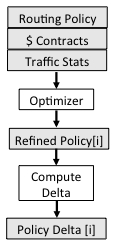
\includegraphics[width=.15\textwidth]{figures/cost-optimizer}
\caption{Optimization architecture}
  \label{fig:optimizer}
  \vspace{-1em}
\end{wrapfigure}

In order to implement these richer policies, we plan to build on top of our other infrastructure,
as shown in Figure~\ref{fig:optimizer}.  The main inputs to the system are (1) a conventional
\Name specification, which determines a \emph{set of allowed routes}, (2) a set of contracts, which
define transit costs, and (3) traffic statistics.  These inputs are fed into an optimizer and
its output is a \emph{refined} \Name specification
for each time period (the $i$ in the diagram refers to the $i^{th}$ time period).
Intuitively, because the user's input specifies a \emph{set} of possible routes, the optimizer is
free to choose exactly which among the possibities are actually used and to vary the choices over time.  
The refined specification represents the particular choice of routes for that time period.  
Once a refined specification has been determined, the difference (delta) between the current
specification and this specification is computed.  The result of compiling the delta will be
pushed to the switches.

We plan to tackle the wide variety of challenges involved in implementing such infrastructure.
When it comes to optimization, we plan to lean on past work 
of Goldenberg~\cite{Goldenberg:multi-home} and others for optimizing multi-homed networks.
When it comes to managing update of router configurations, we will study the right kind
of \emph{consistent update}~\cite{reitblatt+:consistent-updates,Katta:incremental-consistent,Jin:dynamic-updates,McClurg:update-synthesis,McClurg:event-driven-network-programming} to avoid problems that can
occur during update of router configurations.  In particular, we hope to exploit work by 
Francois and others~\cite{FCDB07,CMPFB13} on avoiding packet loss or transient increases 
in network latency when updating BGP or OSPF.  

Finally, while our optimization tools will provide a system for minimizing cost, operators may have 
other non-standard, time-varying objectives.  In order to provide them with the control needed to 
implement these objectives directly, we will develop new \emph{dynamic} abstractions in \Name.  
More specifically, we plan to explore the idea of \emph{time-varying policies}---that is, 
routing policies expressed declaratively as \emph{functions of time and traffic volume}.  We 
also plan to expand the kinds of routing preferences available to programmers 
by allowing \emph{soft preferences},
which admit the possibility that excess traffic may spill over to lower preference routes,
under certain conditions.  Such preferences will generalize \Propane's existing \emph{hard preferences}, whereby lower preference routes are only used in case of failure.

%Initially, we do not plan research on new optimization techniques, though, of course, we will
%pursue such research opportunistically when appropriate.  Rather, we will rely on past research on
%optimization algorithms that balance cost and performance~\cite{Goldenberg:multi-home}.  Such work
%defines both online and offline algorithms.  We will experiment first with the online algorithms 
%that do not assume a priori knowledge of traffic statistics, as they can be applied more easily.

%% \dpw{xxxxxxxxxxxxxxxxxxxx}

%% Many networks have complex business relationships with their peers, providers and 
%% customers~\cite{routingplaybook}, which in turn lead to complex policies that strive to minimize cost and maximize profit.  The \Propane language is not expressive enough to specify these policies.  We plan to explore novel language features to enable their expression in \Name.

%% Consider two policy patterns used in practice and described in the Internet Peering Playbook~\cite{routingplaybook}.   
%% In the {\em fusillade} pattern, a customer network spreads bursts of traffic across five providers, one at a time.  This is done because the customer is billed using the common 95/5 contract, wherein traffic is measured at 5-minute intervals and is billed according to the
%% volume measured during the 95th percentile interval each month.  The fusillade pattern minimizes the volume at the 95th percentile for each provider, while possibly
%% dramatically exceeding this volume when bursting in the 96-100 percentile intervals.
%% In the {\em end-of-month} pattern, a customer network has two providers $P1$ and $P2$ and normally splits traffic between them.  However, the customer has a minimum amount of traffic that it is charged for every month by provider $P2$.   Thus by the end of the billing period, if the total traffic from the customer to the provider falls below this floor, the customer should exclusively use provider $P2$ until the bound is exceeded.

%% To express these kinds of policies, we plan to design an abstraction for specifying {\em dynamic preferences} in \Name, whereby policies can depend on network dynamics.  For example, the fusillade policy requires that each provider be preferred in turn for a set period of time.  The end-of-month policy requires path preferences to change based on time as well as the amount of traffic in the current month.  This idea naturally generalizes \Propane's notion of path preferences, which implicitly depend on a single aspect of network dynamics, namely failures.

%% Implementing such policies will require substantial research.  
%% Our current platform compiles to BGP, 
%% but BGP does not contain mechanisms for processing quantitative information or managing
%% traffic engineering mechanisms.  One implementation strategy we will investigate
%% involves building a controller to monitor traffic levels and pushing BGP
%% updates to switches periodically.  While doing so, we will investigate mechanisms to
%% avoid perils such as route flapping or oscillation.  A second implementation
%% strategy will use a wider range of network devices to implement our strategy,
%% such as switches running OpenFlow~\cite{openflow}, P4~\cite{P4} or PIFO~\cite{pifo}.
%% In the following section (back-end diversity), we describe our complementary efforts 
%% to synthesize configurations
%% for a wider range of protocols and devices in support of high-level \Name policies.  

%% Inspired in part by past domain-specific languages for specifying contracts for financial derivatives~\cite{spj+:contracts},
%% we will also develop a \emph{sub-language} that allow users to specify the
%% \emph{costs} associated with using different interdomain routes, the \emph{peering agreements} they
%% engage in, and the \emph{contracts} signed with customers or providers.  For example,
%% our sub-language will allow description of the two kinds of contracts discussed earlier:  the 95/5 contract as well as 
%% \emph{tiered contracts}~\cite{tiered-isp-contracts}, in which customers promise a certain monthly level
%% of usage in advance in exchange for an improved rate.  Moreover,
%% in addition to \emph{blended contracts}, which charge the same rate for every destination,
%% there sometimes exist different rates for different destinations~\cite{tiered-isp-contracts}.

%% The ability to specify these agreements and contracts can be useful for several purposes.  First, given a matrix of expected traffic along with a \Name policy, we can use the agreements and contracts to automatically estimate the policy's cost, helping \Name users to iteratively refine their cost-aware policies.  Second, we plan to explore the use of search-based optimization strategies to automatically synthesize \Name policies that minimize cost, relieving network engineers of this difficult task.


%% Consequently, we propose using a hetergeneous
%% back-end composed in part of BGP running at the edge, and other mechanisms in the 

%% to handle interdomain
%% routing, and our own custom switch agents, implemented using P4~\cite{p4}, 
%% to manage the traffic monitoring, shaping, policing and routing needed to implement
%% cost-aware routing.  Vargese and Walker both helped design P4 and have considerable experience with it.
%% In addition, in order to optimize cost over a given time period, 
%% such as a month, we will have to update BGP policy dynamically as well,
%% while avoiding perils such as route flapping or oscillation.

%In addition to a new source-level language
%to allow users to specify contracts, we will require new intermediate languages to facilitate implementation of
%our richer policies.  In particular, \Propane's current intermediate language, the PGIR, only allows specification
%of \emph{static} policies---policies that do not change over time.  However, our system will have to include dynamic policies as well as
%traffic monitoring infrastructure.

%In particular,  

%% \paragraph*{Triggers and Time-dependent Routing Preferences}

%% In order to support the large range of policies that real ISPs use, 
%% some of which are detailed in \cite{routingplaybook}, we will invent new abstractions in \Name.   We describe two such ideas, both
%% of which are motivated by policies described in \cite{routingplaybook}.

%% First, at the highest level, \Propane allows the operator to provide a list of routes ordered by preference and to specify that lower preference routes can be used when more preferred routes fail.  Thus in \Propane failure is the only  stimulus for changing a route.  However, a common paradigm is to allow a new route to take over when the amount of traffic volume on what was a high-preference route exceeds a threshold.  Thus, we are led to invent an abstraction and a language construct called a {\em trigger} which includes failures but also other performance related predicates, analagous to a guard~\cite{guardref} in programming languages.  We will need language constructs to model common performance measures that can be used in such triggers such as latency and traffic volume, and statistical measures such as average and 95th-percentile.

%% Next, 

%% It appears to be possible to synthesize both these policies by adding an {\em Optimizer} front-end to the architecture of \Propane that takes as input measured traffic in the past (and predictions for the future), and some choice of objective functions (for example, minimize billed cost).  The Optimizer outputs a set of time-indexed route preferences for a back-end such as the current \Propane system.   Note that while Triggers allow users to manually specify route preference based on performance, the optimizer allows such route preferences to be synthesized automatically.

\paragraph*{Related research.}
There is a vast literature on traffic engineering, much of it designed to avoid congestion 
and minimize cost (see \cite{Awduche:traffic-engineering,Fortz:traffic-engineering,Goldenberg:multi-home}, for
example).  Our research will build upon this work directly; What is new is the design of
compositional high-level \emph{programming languages} that 
specify routes (including inter-domain routes) and financial contracts.
Other recent languages that consider elements of both routing and traffic
engineering include SIMPLE~\cite{simple},
 Merlin~\cite{foster:merlin}, and PANE~\cite{Ferguson:2013}. However, these systems focus on 
specifying capacities, steering \emph{intra}-domain traffic, avoiding congestion and
managing of middleboxes.  They have not tackled 
\emph{inter}-domain routing and optimization for cost-based objectives such as
95/5 contracts signed with multiple ISPs.
Such interactions will lead to different language designs and different implementation
strategies (which mix BGP with traffic engineering mechanisms, for instance).

\paragraph*{Summary of key research questions:}

\begin{itemize}
\item How do we define a specification language that combines inter-domain
routing objectives, fault tolerance and financial contracts?  
%\item It is well known that even the simplest dynamic changes in BGP can lead to timer interactions (for example in Route Flap damping~\cite{routeflapdamping}.  How do we steer away an automatic optimizer from such perils?
\item What are the right abstractions for managing each component of our implementation: 
the optimizer, the time-varying policies, the run-time system and update mechanisms?  
\item What data structures and optimization algorithms, compilation algorithms,
and dynamic route update mechanisms maximize both system performance (compile times and scalability)
and network performance (cost, utilization, and latency)?
\end{itemize}

\subsection{Back-end Diversity}
\label{sec:diversity}

The original \Propane prototype used BGP as a back-end because it is ubiquitous and
could, in principle, handle both inter-domain and 
intra-domain routing.  However, other protocols offer a range of other properties
such as better convergence times and superior quality of service or load balancing that network operators 
will want to exploit.  
%
% \paragraph*{Traditional Protocols.}  
Indeed, most networks use
eBGP to communicate with neighboring networks and 
then iBGP, OSPF or another IGP protocol to distribute routes internally.
Some recent networks also use SDN capabilities.
While BGP operates using local preferences, filters and community values,
some protocols such as OSPF
use real-valued link weights to compute shortest paths, which are not
supported in \Propane.  
%In addition, in order to support scalability, 
%an OSPF network may be divided into separate \emph{areas} that only selectively
%export shortest paths information --- here, there is a tradeoff between 
%convergence time and finding optimal paths.  
If \Name cannot synthesize configurations that take advantage of available
back-ends and their performance properties, 
operators will be reluctant to deploy the system.

The central technical challenges involved in generation of multiple back-end protocols, involve
extending our key intermediate languages to enable representation 
of these additional features (\eg, link weights, OSPF areas, static routes,
route redistribution, \etc).  
In addition to changing our intermediate representation, we will also need to 
change our internal safety analysis algorithms to reflect the semantics of 
link weights and other new features.
Some additional challenges include deciding exactly which protocols should be used,
as well as how and where
a synthesis algorithm should divide a network into OSPF areas.  We will also
explore extensions to the \Name front end language to give users
control over such features.
Finally, our synthesis algorithms will have to manage the interactions
\emph{between} protocols --- interactions between protocols via route redistribution
is surprisingly tricky and can easily lead to unexpected routing loops~\cite{cisco-route-redistribution}.
Past tools for control plane synthesis, including \Propane, have not been formalized or proven correct. 
In order to defend against such problems and to ensure the reliability of our tools, we plan to formalize 
our techniques using programming language
theory (using similar techniques to those employed in research on NetKAT~\cite{netkat} or BagPipe~\cite{bagpipe}), and prove their correctness
rigorously.

\paragraph*{Related Work.}
ConfigAssure~\cite{narain:lisa05,narain+:configassure} and DADC~\cite{DADC} are alternative
systems designed to help users synthesize
configurations that involve multiple protocols, such as OSPF and RIP. 
However, ConfigAssure does not 
provide the same kind of high-level abstractions as \Name
(regular paths, predicates, abstract topologies and route preferences) and does not
support inter-domain routing via BGP.  Consequently,
the intermediate languages algorithms used in \Name are quite
different from ConfigAssure, which uses logic programming and SAT.
\Name will also provide different domain-specific analyses, including analyses for
fault tolerance.  Finally, the semantics of ConfigAssure, DADC, and Propane have not been defined formally,
and their algorithms have not been proven correct.

\paragraph*{Summary of key research questions:}

\begin{itemize}
\item How do we reorganize and extend our intermediate languages to encode and
implement new features of various standard protocols such as link weights
or areas in OSPF?  
\item How do synthesis algorithms decide which protocols to use and where?
Which properties (convergence time, scalability?) govern these choices?
\item How does the compiler reason about administrative distances
and the interactions of several different protocols in a single
implementation?
% \item Is it possible to exploit the properties of next generation
% programmable switches, such as those implementing P4,
% to define more complete and efficient implementations of \Name
% rovided this hardware is available?
\end{itemize}

\subsection{Migration Technology and Mixed Verification}

\begin{figure}[t] 
  \centering
  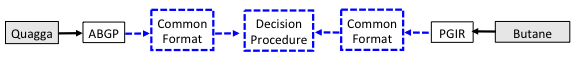
\includegraphics[width=.9\textwidth]{figures/generic-equivalence}
\caption{Architecture for \Name verification and migration technology.}
\label{fig:transition-tech}
\end{figure}

Higher-level policy languages such as provided by the \Name platform provide clear advantages for network understanding, maintenance, and reliability over the low-level style in use today.  
%While network engineers and operators would like to accrue these advantages, they are also hesitant to convert their networks to a new technology, and quite reasonably so.  
However, it costs significant human time and effort to translate low-level configurations into a higher-level policy and to ensure that the original functionality and performance is preserved.  Moreover, migrating all operations at once is typically logistically impossible.   In our discussions with network engineers it has become clear that these issues are key barriers to practical deployment of new approaches to network configuration technology.  To address these problems, we plan to develop automated tools to help network engineers
\emph{correctly} and \emph{incrementally} migrate existing subnetworks to the \Name platform.  In addition, we will
support mixed-mode verification and operations technology so that networks can safely
run a combination of legacy-controlled and \Name-controlled networks.  Mixed-mode operation will not only allow
migration to proceed in a slow, controlled fashion, but will also allow engineers to test \Name on a tiny fraction of their
traffic first to reassure them that the technology is functioning properly.

%% and legacy to help guarantee that \Name can {\em integrate} the \Name technology with existing approaches to support a flexible, hybrid approach to network configuration.

%% Further, an all-or-nothing approach to conversion to \Name is a non-starter for several reasons.  First, it precludes an incremental deployment strategy, whereby subnetworks are converted one at a time.  Second, it precludes a mixed configuration style consisting of both low-level directives and high-level policies.  Such a style allows legacy subnetworks to remain unchanged while enabling new subnetworks to take advantage of \Name.  It also provides an ``escape hatch" for engineers to obtain fine-grained, low-level control over network configuration when the desired behavior is not (easily) expressible in \Name. 




\paragraph{Migration.}  Figure~\ref{fig:transition-tech} sketches our proposed architecture for tool-supported migration 
to the \Name platform.  The high-level idea for our migration plan is that a network engineer will
provide a candidate \Name policy for their network.  That candidate will be compared to
the current low-level network configuration.  In order to perform the comparison, the
high-level and low-level configurations will be converted into a common 
intermediate format, and then a decision procedure that tests for equivalence, and other properties, will be applied.
When the two policies differ, the system will automatically generate
concrete \emph{counter-examples}.  These counter-examples will
include: (1) a network policy environment, including a failure scenario and advertisements
sent from external peers, (2) a concrete packet, and (3) the path each policy causes the packet to take in the given environment.
The engineer will use this information to iteratively revise the 
candidate \Name policy until it achieves the desired correspondence with the legacy configuration.  

In order to implement this ``meet-in-the-middle'' strategy, we plan to use the
fragment of first-order logic supported by 
automated Satisfiability Modulo Theories (SMT) solvers such as Z3~\cite{z3} as the
common intermediate language.  Using this logic as an intermediate language has both the
advantages of great encoding flexibility and also backing by automated decision procedures.
More specifically, our encoding will take 
inspiration from Griffin's work~\cite{griffin+:stable-paths},
which characterizes BGP as a process that solves the \emph{stable paths problem}, 
a generalization of the  \emph{shortest paths problem}.  
%In order to translate both low-level configurations and PGIR graphs into
%logical formulae that represent the stable paths problems being solved.
For instance, the following logical phrases present an idealized sketch of the 
core technique we will investigate (below $x$, $y$, $z$ are routers):
%
\newcommand{\pfont}[1]{\mathsf{#1}}%
%
\[
\begin{array}{ll}
(1) & \pfont{canUse}(x,y) \leftarrow \neg \pfont{failed}(x,y) \wedge \pfont{hasPath}(y) \\
(2) & \pfont{uses}(x,y) \leftarrow \pfont{canUse}(x,y) \wedge \pfont{best}(x,y) \\
(3) & \pfont{best}(x,y) \leftarrow \bigwedge_z \neg \pfont{canUse}(x,z) \vee \pfont{localPref}_x(y) \ge \pfont{localPref}_x(z) 
\end{array}
\]
Clause (1) says $x$ can use a route through $y$ if $y$ has not failed and $y$ has a path to the destination. 
Clause (2) says $x$ actually \emph{does}
use $y$ if it \emph{can} use $y$ and $y$ is its best option (this is the stability clause --- it does not prefer some other
route).  Clause (3) defines what it means for $y$ to be the best option for $x$ --- that for all other options $z$, either
$z$ cannot be used or $x$ prefers $y$ to $z$.  We believe an encoding 
based around this technique will be efficient because it avoids having to reason
explicitly about message ordering.  Instead, it characterizes the possible solutions to the routing problem, which Griffin has shown will be stable paths~\cite{griffin+:stable-paths}.
We plan to implement this encoding and then use an SMT solver to test configurations for a wide range of properties, including equivalence, 
stability, reachability, fault tolerance and other properties of interest to network engineers during the
migration process.  SMT solvers like Z3 will also produce \emph{counter-examples} 
when they cannot prove a formula correct. A secondary
research problem is to develop techniques for massaging the counter-examples produced by Z3 into a form to present
to a network operator.  

%% We have already begun to experiment with this encoding and our initial tests suggest
%% that these techniques will scale to moderate-sized networks with at least 100 routers or
%% more, depending on the network policies and properties of interest
%% (and hence will be applicable to the majority of corporate and campus networks
%% that do not exceed this size).  To scale to larger data-center sized networks,
%% we plan to investigate integrating these SMT-based techniques with
%% Varghese's techniques involving symmetry and surgery~\cite{bjorner+:scaling-network-verification} as well as the topology
%% abstractions described earlier in this proposal.



%% First, we must convert both the low-level configurations and
%% higher-level policy to a common representation.  As shown in the figure, we
%% plan to use our graph-based PGIR representation for this purpose, as it is a
%% powerful context-sensitive representation that makes all allowed paths
%% through the network explicit.  While conversion from vendor-specific
%% configurations to the vendor-neutral ABGP format should be technically
%% straightforward, the conversion from ABGP to PGIR is non-trivial due
%% to the expressiveness of BGP policies.  Key elements of BGP policies
%% include regular expression (and other) filters, complex local
%% preferences and the use community tags.  Each of these features 
%% must be translated into an equivalent PGIR
%% representation in order to develop a robust migration tool.  We
%% believe we can handle regular expression filters via translation to
%% automata, whose graph-like structure may be represented directly as a
%% PGIR subgraph. Arbitrary community values may be processed by encoding
%% the set of valid communities attached to an advertisement in the PGIR
%% nodes.  Local preferences may be handled via the PGIR's preference
%% mechanisms.  However, implementing an efficient algorithm to
%% manage translation of all of these mechanisms at once, and proving it correct, will take significant
%% research.  In addition, in the later years of the project, we will
%% extend our migration tools to handle additional protocols such as OSPF
%% and RIP.  As suggested in Section~\ref{sec:diversity}, doing so will
%% require extensions to the PGIR with link weights, and, of course, new
%% algorithms that we plan both to implement and to explore theoretically
%% via proofs of correctness.

%it does not suffice to simply ``invert" \Name's current translation from PGIR to ABGP, since that translation generates stylized ABGP configurations
% which in our experience differ in important ways from manually written configurations.  We will instead identify common BGP idioms that network engineers use to enforce different aspects of network behavior and then develop translation strategies that target these idioms.  We may also be able to leverage a comprehensive model of low-level configurations that was developed in our prior work~\cite{}.

%% Once both the low-level configuration and higher-level policy have been 
%% converted to a common representation, we must compare the two resulting
%% PGIRs for equivalence, or perhaps show that one (the low-level configuration)
%% is a faithful implementation of the other (the higher-level policy).  Alternatively,
%% if the two policies are incompatible,
%% we might produce a counter-example---a packet that
%% is treated differently by the two PGIRs, which the network operator may use
%% to debug the policy.  One possibility is to generate our own custom equivalence
%% algorithm over these structures.  A custom algorithm has the potential to exploit
%% domain-specific heuristics for performance.  However, we will begin our research instead
%% by looking at encodings of PGIRs and the equivalence question in logic
%% and applying an off-the-shelf
%% Satisfiability Modulo Theories (SMT) solver such as Z3~\cite{z3}.  Such solvers
%% are often used to answer equivalence and other verification questions.  When
%% verification fails, they will report counter-examples, which our system  We would have to take
%% We can then
%% ask the SMT solver to prove that the two policies are equivalent or
%% otherwise produce a counterexample, which corresponds to We also determine the full
%% path the network that the packet takes under each policy and present
%% that to the user, allowing him to easily understand the differences
%% and make appropriate changes to the \Name policy.

One downside of the proposed approach is that it requires the engineer
to devise an initial \Name policy manually, which the migration tool
then helps to iteratively improve.  In the later portions of the project, 
we will also consider approaches to \emph{partially} or 
\emph{completely} {\em infer} a \Name policy directly from the given
low-level configuration.  One approach to partial inference is
to allow a user to provide a \emph{sketch}~\cite{sketch} of a policy,
which is a policy containing some ``holes'' that the system will fill in
automatically.  Following earlier work by Solar-Lezama~\cite{sketch}
in other synthesis domains, we can convert this sketch into an SMT formula
(using the intuitions described above)
and look for satisfying solutions that make it equivalent to 
the existing low-level configuration.
%Such SMT-based synthesis procedures have been highly effective in other domains.
A second approach we will investigate involves focusing on inferring \Name's
high-level abstractions more directly.  In particular, \Name's core policies are
phrased in terms of regular expressions and there are a variety of algorithms
in the literature, such as the L* algorithm~\cite{Angluin87} that may be used to
infer regular expressions.
%expressions to specify allowed paths, is to expoit
%existing algorithms for learning regular expressions.
%For example, the L* algorithm learns regular expressions given a
%``teacher" that can answer membership and equivalence queries~\cite{}.
%In our setting, we can simulate the teacher by querying the PGIR
%representation of the low-level configuration, as well as by
%interaction with the user.  
However, we will likely need to extend such
learning algorithms to handle other aspects of \Name, such as its
support for prioritized paths.

\paragraph{Mixed Operation and Verification} There are several challenges in supporting a mixed form of configuration, whereby some portions of the network behavior are specified with \Name and some using existing technologies.  Currently the \Propane platform guarantees by construction that produced low-level configurations faithfully implement the high-level policy, and furthermore that this policy will be respected in the face of arbitrary failures.  The inclusion of existing low-level configurations for some portions of the network significant complicates the ability to provide these guarantees and any others that we may want to augment the platform to support. First, the \Name compiler has less flexibility because it must retain the given low-level configurations as is.  Second, the \Name platform must be able to reason about the network as a whole despite the fact that portions are manually configured.

To address these challenges we plan to adapt ideas from the literature on compositional program analysis and verification.  In particular we will leverage the notion of {\em assume-guarantee reasoning}~\cite{Jones:assume-guarantee,Pnueli84}, which allows components to be analyzed separately in order to ensure global properties of interest.  In our setting, we will require {\em interface specifications} for the manually configured portions of the network. 
The \Name platform then can {\em assume} that these specifications hold when reasoning about the network as a whole and compiling the \Name-specific portions.  Separately, we must {\em guarantee} that the manually configured portions indeed meet their interface specifications.
Such interfaces could specify the property that, for example, a legacy OSPF configuration establishes full-mesh connectivity.  A
\Name-controlled BGP configuration might depend upon full-mesh connectivity to implement inter-domain routing correctly.
Alternatively, an interface might guarantee isolation properties of subnetworks so their
operation does not interfere with one another. In general, interfaces 
describe {\em abstractions} of low-level configurations that are relatively simple to reason about, yet precise enough to allow the platform to compile the remaining \Name policy while providing strong correctness guarantees.
We believe we can exploit a wealth of ideas from the program analysis community on sound forms of abstraction
to help generate such interfaces. 
%for various properties of interest (e.g., overapproximations vs. underapproximations), along with techniques such as counterexample-driven refinement for incrementally improving candidate abstractions..

%Several questions must be answered to make this approach effective and practical.  What is the form of interface specifications?  How are they produced?  How are they verified?  How must the \Name platform's analysis and compilation algorithms be modified to accommodate these specifications?  As a first cut, a natural choice is for interface specifications to be written in the \Name policy language itself.  We can then leverage similar ideas as described above in the context of migration in order to produce and/or validate these specifications relative to existing low-level configurations.  

%, in the migration setting the goal is to infer {\em equivalent} \Name policies for low-level configurations.  In contrast, here that goal may not be possible due to expressiveness limitations of \Name, and furthermore it is not desirable even if it is possible. Rather, 

%% More generally, interfaces describe {\em abstractions} of low-level configurations that are relatively simple to reason about, yet precise enough to allow the platform to compile the remaining \Name policy while providing strong correctness guarantees.  Here we can leverage a wealth of ideas from the program analysis community on sound forms of abstraction for various properties of interest (e.g., overapproximations vs. underapproximations), along with techniques such as counterexample-driven refinement for incrementally improving candidate abstractions.


%% As a simple example, consider a subnetwork whose low-level configurations involve a sophisticated load balancing scheme via a form of multipath routing.  It is not useful to attempt to exactly represent this complex scheme in the language of \Name, and indeed it may not even be possible.  Rather, it suffices for the \Name policy to express the {\em possible} paths that each packet can take, along with any backup paths to use in the case of failures.

%Finally, given an appropriate interface specification for manually configured portions of the network, we must generalize the \Name compilation strategy to incorporate the assumption that those portions meet their specifications as well as the constraint that those configurations cannot be modified.


% \begin{wrapfigure}{R}{0.5\textwidth}
%   \centering
%   \small
%   \begin{tabular}{|l|l|l|l|l|}
% \hline\hline
% {\bf Protocol} & {\bf Feature} & {\bf ERA} & {\bf ARC} & {\bf Prop} \\\hline\hline
% OSPF & Single area & Yes & Yes & Yes \\
% & Multiple areas & ? & ? & Yes \\ \hline
% eBGP  & Local pref & Yes & No & Yes \\
%   & RE filters &  No & No & Yes \\
%   & Communities & No & No & Yes \\\hline
% iBGP & & No & No & Yes \\\hline
% %Route & Acyclic & Yes* & Yes* & Yes \\
% %Redistrib.  & Cyclic & Yes* & No & Yes \\
% %& \multicolumn{3}{|l|}{* ERA and ARC are unsound.} \\
% %& \multicolumn{3}{|l|}{For example: \cite{cisco-route-redistribution-tricky} \\
% %Aggregation & Black holes & No & Maybe \\\hline 
% \hline
% {\bf Property} & {\bf Variant} &  &  &  \\\hline\hline
% Equivalence & & No & Yes & Yes\\\hline
% %Preferences & & No & No & Yes\\\hline
% Stability & Unique & No & No & Yes \\
%  & Wedgie & No & No & Yes \\\hline
%   \end{tabular}
% \caption{ERA and ARC vs proposed work (Prop). }
% \label{fig:smt-vs-arc}
% \end{wrapfigure}

\paragraph*{Related research:}  
One way to realize the migration architecture in Figure~\ref{fig:transition-tech} is to compile the \Name policy into a low-level configuration
and then to use existing tools for configuration analysis~\cite{batfish,arc,bagpipe,era} to compare the two low-level configurations.  This is a reasonable approach, but much additional research is required before existing
tools are powerful enough to achieve our migration goals.  Specifically, all existing configuration analysis tools have important limitations that would prevent their usage in our context.  Batfish~\cite{batfish} and ERA~\cite{era} can find configuration bugs in the context of a specific user-specified environment (i.e., a particular failure scenario and set of route announcements from neighboring networks) but cannot verify configurations on \emph{all} possible environments.  ARC~\cite{arc} soundly reasons about certain properties in the context of all possible failures but not all possible route announcements; Bagpipe~\cite{bagpipe} has exactly the opposite limitation.  In addition, many of these tools are limited in the router
features that they support --- for instance, ARC does not support core BGP features such as
general local preferences, community values, or regular expression filters, all of which
\Name needs.
%Further, these tools are targeted at checking properties of a single configuration, while we require the ability to compare the behaviors of two configurations to one another.

There is also a great deal of work on verification of a specific incarnation of the network as embodied by its \emph{data plane} (forwarding tables), such as work on AntEater~\cite{mai+:anteater}, Header Space Analysis~\cite{hsa},
Veriflow~\cite{khurshid13veriflow}, Network Datalog~\cite{nod} and many others.  This work is fundamentally different from our
verification needs, which requires reasoning about the network's \emph{control plane} as specified in its configuration.

\paragraph*{Summary of key research questions:}

\begin{itemize}
\item How do we translate low-level configurations into logical representations?  Can these logical representations be used
for equivalence testing and verification of other important properties?  To what extent does this technique scale?

\item How do we automate generation of counter-examples? What form should user feedback take?

\item Can SMT-based synthesis or RE-learning techniques help us infer \Name policies directly from low-level configurations given a partial \Name polic or no \Name policy at all to start from?

\item What form of interface specification is necessary for a manually configured subnetwork, in order to support safe mixed-mode \Name analysis, compilation and operation?

\end{itemize}





%% \section{Related Work}

%% To reduce configuration errors, operators are increasingly adopting an
%% approach in which common tasks are captured as parameterized templates~\cite{hatch,thwack}.
%% %
%% %More powerful still are systems like
%% %ConfigAssure~\cite{narain:lisa05,narain+:configassure}, which use SAT solving
%% %and model finding tools to fill in parameters in configurations while
%% %ensuring key correctness constraints are satisfied.
%% %One step further, systems like
%% %ConfigAssure~\cite{narain:lisa05,narain+:configassure} use SAT solving
%% %and model finding tools to correctly and consistently fill in some parameters.
%% %
%% While templates help ensure certain kinds of consistency across devices,
%% they do not provide fundamentally different abstractions from existing configuration languages
%% or bridge the semantic divide between network-wide policies and device-level configuration.
%% %They do not provide fundamentally different abstractions
%% %from existing configuration languages and
%% Thus, they still require operators to
%% manually decompose policies into device behaviors and to reason manually about the interaction of different
%% protocols.

%% As a complementary approach, configuration analysis tools can help
%% reduce misconfigurations by checking if low-level configurations match
%% high-level policy~\cite{batfish,feamster+:rcc}. However, such tools, while
%% an important component of any network management system,
%% cannot, on their own, help operators with the challenging task of generating
%% configurations in the first place.

%% %Further, today's tools cannot verify correctness under concrete failure scenarios, rather than under all possible failures.

%% Software-defined networking (SDN) and its abstractions
%% are, in part, the research
%% community's response to the difficulty of maintaining policy
%% compliance through distributed device interactions~\cite{ethane}.
%% Instead of organizing networks around a distributed
%% collection of devices that compute forwarding tables through
%% mutual interactions, the devices are told how to
%% forward packets by a centralized controller. The controller is responsible for ensuring that the
%% paths taken are compliant with operator specifications.
%% %Researchers
%% %have developed increasingly sophisticated languages that let operators
%% %specify desirable network paths~\cite{x,y,z} which are then translated
%% %to forwarding tables at runtime.



\section{Broader Impacts of the Proposed Work}
\label{sec:impact}

The proposed work, if successful, has the potential to transform the way
that thousands of networks in the US and all over the world are managed.
By developing higher-level, correct-by-construction abstractions for
network operators, and creating a path to deploy those abstractions
in real networks, the \Name platform will decrease
errors in network policy design and implementation, and subsequently
to decrease network downtime and vulnerability to attack.  However,
for maximum impact, we need to engage in both industrial outreach and
educational activities.

\paragraph*{Cloud Deployment.} 
We will work with the operators of two major clouds, Microsoft Azure and Google, to test our language and system using the policies of real industrial networks, to identify the pragmatic barriers to adoption, and to deploy our system where possible.
All three PIs have a strong connection with Microsoft. Walker, via PhD student Ryan Beckett, and MSR collaborators Jitu Padhye and Ratul Mahajan, translated a number of Azure policies into Propane in 2015 and validated his models with Microsoft operators. Millstein has collaborated with networking researchers at MSR for the last ten years and recently won an MSR Outstanding Collaborator Award. As part of this collaboration, Millstein's Batfish~\cite{batfish} tool identified several configuration errors in Azure data centers that were subsequently fixed. Varghese worked at MSR from 2012-2016 and continues to collaborate with his former colleagues. We will also work with Google.  Both Walker and Varghese have collaborated with Amin Vahdat, the head of networking in the past. These two clouds are different because Azure is a public cloud while the Google cloud supports Google services; adding abstractions that cover both use cases will be an important step toward credibility. Collaboration will be facilitated via student internships at Microsoft and Google, as we have done recently with Princeton and UCLA Ph.D. students Ryan Beckett and Ari Fogel.  See attached letters of collaboration.

\paragraph*{Industrial Outreach.}
In 2016, the networking and programming languages
researchers at Cornell and Princeton universities 
formed the Cornell-Princeton Center for Network 
Programming (CNP)~\cite{center-for-network-programming}.
While there is a large an vibrant networking community on the US
West Coast, centered in the Bay Area, there was no such community on
the US East Coast.  The CNP was formed to create such a community.
Our first major event was a 1-day workshop held in June 2016 at
Cornell Tech in New York.  It included roughly 50 participants from
academia and a wide array of businesses in the New York area including
Cisco, Juniper, Huawei, Intel, Goldman Sachs, Verizon, Google, Amazon,
Yahoo and many more.  The workshop included technical presentations by
academics, panel discussions with industry experts, and many breaks to
facilitate small group conversation.  The workshop fulfilled its aim
of allowing academics and industry to exchange problems and solutions,
vision for the future, and contact information for follow-up
discussions. We propose to organize a future meeting of this form
under the CNP umbrella and the auspices of this grant.  PI Walker will
organize the logistics and PIs Varghese and Millstein will attend and
give talks on their research.

\paragraph*{Educational Initiatives.}
In addition to disseminating our ideas to industry today,
we need to begin educating the network operators and engineers 
of tomorrow.  Such engineers will need a mix of skills that include
both knowledge of networking protocols and knowledge of formal methods.
With that in mind, we plan to develop new modules for networking courses
at both the graduate and undergraduate level.  
Such modules will have
several goals: (1) To teach both low-level mechanisms and high-level abstractions;
(2) To introduce a range of \emph{rigorous}, \emph{formal} properties of
 interest; (3) To expose to students to basic algorithms for verification of such
properties.
In addition to teaching concepts, we will give students hands-on
experience writing policy using our language and verification tools.  
More specifically, we plan to develop online tutorials for our tools
that we can use in our classes.  To do so effectively, we will
integrate our work with the CORE simulator~\cite{core}.  CORE
will allow students to visualize, experiment with, and test their
use of our specification language and verification tools.
Varghese and Millstein have already begun developing a curriculum for this initiative
by co-teaching a seminar class at UCLA in Fall 2016 on ``Verification, Synthesis, and the Creative Habit'' 
and plan to use this experience to create a formal graduate class.  PI Walker will work with
his colleague and long-time collaborator Jennifer Rexford to integrate modules tested by Varghese and Millstein into Princeton's
graduate and undergraduate networking courses.

In addition to traditional in-classroom teaching, the PIs have a strong 
track record of mentoring
undergraduate research projects.
The PIs will
investigate the use of REUs to provide additional undergraduate opportunities, and they will continue to make use of existing programs at their universities. For example, Millstein has mentored multiple undergraduates on research through UCLA's Cross-disciplinary Scholars in Science and Technology program\footnote{\url{http://www.csst.ucla.edu}}.
Millstein has also mentored several promising high-school students on research through UCLA Engineering's High School Summer Research program\footnote{\url{http://esc.seas.ucla.edu/high-school-summer-research-program}}.

\paragraph*{Under-represented minorities.} The PIs are dedicated
to, and have a track-record of, providing opportunities to women and under-represented 
minorities.  For instance, two of Walker's past undergraduate advisees,
Lester Mackey (African American) and Katherine Ye, won the CRA undergraduate 
outstanding undergraduate
research award.
%% For example, PI Walker has mentored two winners of the CRA
%% outstanding undergraduate award, and both happened to be
%% under-represented minorities in computer science: one an African
%% American student and one a woman.  The former, Lester Mackey, went
%% on to get his Ph.D.\ in computer science, and the latter, Katherine
%% Ye, started graduate school in Fall 2016.  
Millstein co-advised female Ph.D.\ student Nupur Kothari (now at Microsoft) for her dissertation on analysis of networked systems and currently advises one female Ph.D.\ student (Lun Liu).  Varghese has mentored several women, including
co-advising Lili Qiu (now a professor at UT Austin) and Lavanya Jose (currently a graduate student at Stanford).
The PIs will work to continue to seek out under-represented minorities and provide exciting 
research opportunities for them.

\section{Results from Prior NSF Support}
\label{sec:prior-support}

\noindent
{\bf David Walker, PI. NSF CNS-1111520, Intellectual Merit:}
In NSF CNS-1111520, \emph{High-Level Language Support for Trustworthy Networks}
(\$1,400,000, 08/11-08/16),
PI Walker and his collaborators developed new languages, interfaces
and systems for managing software-defined networks (SDNs).  
This project produced the Frenetic family
of network programming languages, the first high-level languages for
programming software-defined networks.  These languages, which include
Frenetic~\cite{frenetic}, 
Pyretic~\cite{pyretic},
NetKAT~\cite{netkat} and others, all adhere to the
\emph{principle of compositionality}, a key design element missing
from earlier network programming languages.  
%They also invented the
%notion of consistent network update~\cite{reitblatt+:consistent-updates},
%which ensures key safety invariants are preserved across network update.
Open source code for systems produced by this project is available
at \url{frenetic-lang.org}.
%
{\bf Broader Impacts:} 
The PIs held a well-attended summer school on network programming and 
verification for students and faculty. The
Pyretic programming language was used in Nick Feamster's popular
SDN MOOC; thousands of students and
network operators all over the US used it to learn principles of network
programming.  The PIs
also helped create the P4 switch configuration language~\cite{P4}, which is
becoming an industry standard.

\medskip
\noindent
{\bf Todd Millstein, PI. NSF CNS-1161595, Intellectual Merit}: In NSF CNS-1161595, {\em NeTS: Medium: Collaborative Research: Systematic Analysis of Protocol Implementations} (\$446,860, 5/12--4/17), PI Millstein and collaborators developed techniques for automatically testing and verifying properties of network protocols and configurations.  Our PIC tool leverages and extends symbolic execution techniques to automatically identify subtle interoperability errors in network protocol implementations~\cite{DBLP:conf/nsdi/PedrosaFKGMM15}.  Our Batfish~\cite{batfish} and ERA~\cite{era} tools employ novel logical models of a network's control plane to verify properties of low-level network configurations.  This award also partially funded Millstein's work on the Propane network programming language~\cite{beckett+:propane}. 
%
{\bf Broader Impacts:} PIC, Batfish, ERA and Propane are all publicly available and open source on Github.  PIC identified several previously unknown interoperability errors in popular implementations of the SIP and SPDY protocols, many of which were fixed by the developers.  Similarly, Batfish identified dozens of misconfigurations in the campus networks of two large universities as well as the data-center networks of a large cloud provider.

\noindent
{\bf George Varghese:} Varghese has been awarded 10 NSF grants, but none in the last 5 years 
as he worked in industry.  Past grants led to innovations such as Deficit Round Robin, IP lookups and worm fingerprinting.

%%% Local Variables:
%%% mode: latex
%%% TeX-master: "proposal.tex"
%%% TeX-PDF-mode: t
%%% End:
